\documentclass[../Bachelorarbeit.tex]{subfiles}
\begin{document}
\chapter{Stand der Technik}
\label{chap:analyse}

Nachdem in Kapitel \ref{chap:einfuehrung} - \nameref{chap:einfuehrung} die ersten konkreten Überlegungen bis hin zu einem \nameref{sec:anwendungsszenario} aufgezeigt wurden um den Inhalt und die Funktionsweise des Prototypen zu umreißen, widmet sich dieses Kapitel der Domäne für die der Prototyp entwickelt wird.
Für diesen Zweck ist das Kapitel in zwei Abschnitte unterteilt. 
Im ersten Abschnitt (\nameref{chap:analyse:sec:sota}) wird ein Blick auf die Forschung und Fachliteratur geworfen, während sich der zweite Abschnitt (\nameref{chap:analyse:sec:analyBestehendeKonz}) mit echten Projekten beschäftigt, die eine Relevanz für den Prototypen darstellen.


\section{Literaturrecherche}
\label{chap:analyse:sec:sota}


\ideas{Einführung Themen aus der Entscheidungstheorie...Einzelne Punkte von Tufte, je nach Relevanz...Literaturrecherche ... sowie was aktueller Stand der Technik sowie Forschung.}



Daten OSM

\todoImprovement[]{weitere Analyse}
\todoInfo[]{Was ist gut, was ist schlecht?}

\section{Analyse von bestehenden Konzepten}
\label{chap:analyse:sec:analyBestehendeKonz}
\todoImprovement[]{Abschnittstitel konkretisieren}
\todoImprovement[]{Thema genauer ausarbeiten}


\subsection{Google Maps}
\label{chap:analyse:sec:sota:sec:google_maps}


\subsection{Airbnb}
Bei Airbnb handelt es sich um eine Webseite die sich auf die Vermittlung von Unterkünften spezialisiert hat\footnote{
	Airbnb ist unter der Addresse https://www.airbnb.at zu erreichen. Die getätigten Aussagen über die Webseite beziehen sich auf den Stand von Sommer 2016.
	}. 
Dabei können sich gastgebende Personen registrieren und Übernachtungsmöglichkeiten von einem Zimmer bis hin zu ganzen Immobilien anbieten. 
Anhand diverser Such- und Filterkriterien ermöglicht die Webseite den Suchenden eine passende Unterkunft zu suchen und diese über die Webseite zu reservieren.
Neben klassischen Bewertungen bietet die Webseite auch Social Media Komponenten wie Profile, das hochladen eigener Fotos und das liken  sowie die Möglichkeit sich als gastgebende Person eine eigene Marke aufzubauen (vgl. \cite{Yannopoulou2013}, S. 3).

\subsubsection*{Aufbau von Airbnb}
Nachdem auf der Startseite die gewünschte Stadt in der man übernachten möchte, sowie optional das Start- und das Enddatum, ausgewählt wurden wird man auf die eigentliche Seite zur Planung weitergeleitet (siehe Abb.: \ref{fig:airbnbOverview} - \nameref{fig:airbnbOverview}).
Die Planungsansicht unterteilt sich in die drei Bereiche Auswahlkriterien/Filter, Rasteransicht der Ergebnis sowie der Kartendarstellung.
Die jeweiligen Bereiche sind durch unterschiedliche Farbgebungen des Hintergrundes klar voneinander abgetrennt.

\paragraph{Auswahlkriterien/Filter}
\label{airbnb:filter}
Die Ansicht des Bereichs kann der Abb.: \ref{fig:airbnbOverview} - \nameref{fig:airbnbOverview} entnommen werden und wird durch den roten Rahmen mit der Nummerierung 1 markiert (links oben).
Durch Änderungen in diesem Bereich werden die beiden anderen Bereiche (\nameref{airbnb:gridview} und \nameref{airbnb:map}) automatisch aktualisiert. 
Dieser Bereich ist in der Standardansicht in vier Zeilen aufgeteilt. 
In der ersten Zeile (ganz oben) befindet sich ein Textfeld welches Standardmäßig die zuvor ausgewählte Stadt/Region anzeigt. 
Sobald man das schreiben im Textfeld beginnt, wird man bei der Eingabe durch eine Auswahl passender Einträge unterstützt, welche unter dem Textfeld eingeblendet werden.
Mithilfe der zweiten Zeile von oben lassen sich die optionalen Daten von der Startseite (Start-, Enddatum und Anzahl der Gäste) nachtragen oder ändern.
Die Art der Unterkunft wird mit Hilfe der dritten Zeile von oben ausgewählt.\\
\\
In der vierten Zeile von oben werden die Preise mit Hilfe eines stilistischen Balkendiagramms angezeigt. Dabei verlaufen die Preise ansteigend auf der X-Achse.
Die Information über die Anzahl der Unterkünfte in der entsprechenden Preisklasse wird mithilfe der Y-Achse schematisch dargestellt
\footnote{Die genau Information kann aufgrund der fehlenden Beschriftung der Y-Achse oder einer anderen visuellen Unterstützung nicht abgelesen werden.
	}.
Mithilfe von zwei Schiebereglern kann die untere- und obere Grenze für die Preisspanne festgelegt werden, der jeweilige Betrag wird direkt unter den Reglern dargestellt.
Zusätzlich wird der durchschnittliche Preis der Region/Stadt unter der Preisspanne dargestellt.\\
\\
Mit einem klick auf den Button Filter (siehe Abb.: \ref{fig:airbnbOverview} - linke Seite zwischen oberen- und unteren roten Rahmen) wird der Bereich \nameref{airbnb:filter} expandiert und überlagert die  \nameref{airbnb:gridview}.
Dabei ist aufgefallen das die Platzierung des Buttons für mich etwas irritierend wirkt. 
Wie zuvor erwähnt, werden die einzelnen Bereiche durch die unterschiedliche Farbgebung des Hintergrundes abgegrenzt. 
Dabei befindet sich der Button Filter im grauen Bereich (\nameref{airbnb:gridview}) wenn man allerdings darauf klickt wird der expandierte Bereich in der hellen Hintergrundfarbe des \nameref{airbnb:filter}-Bereichs dargestellt.


\begin{figure}[H]
\centering
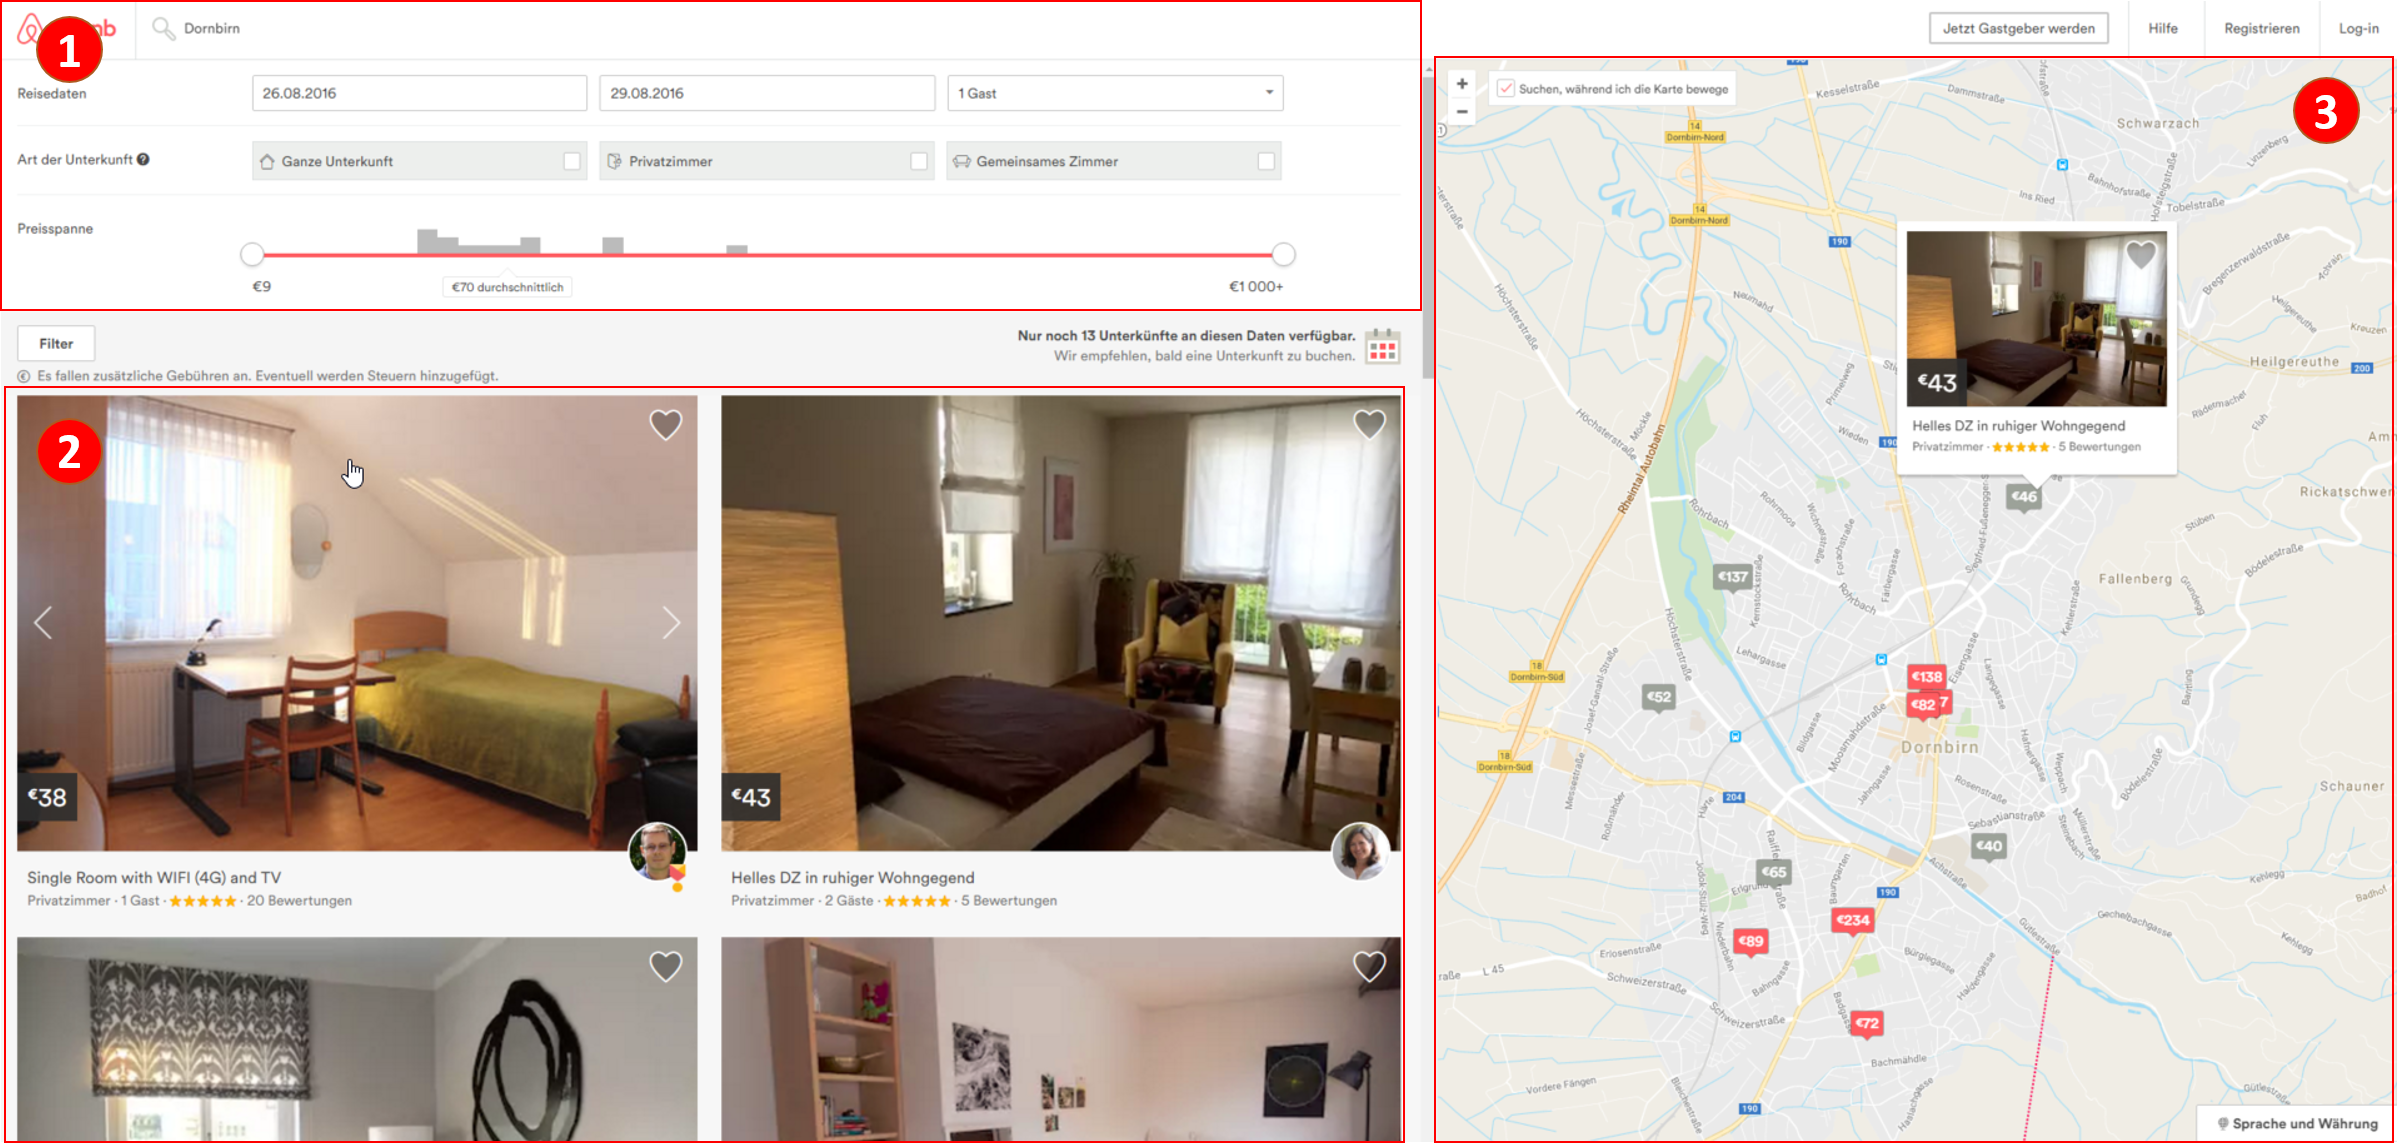
\includegraphics[width=1\linewidth]{img/StandDerTechnik/airbnbOverview}
\caption[Übersicht: Aufbau von Airbnb]{Übersicht: Aufbau von Airbnb (Quelle: eigene Ausarbeitung | Daten und Kartenmaterial: https://www.airbnb.com/ - Stand Sommer 2016)}
\label{fig:airbnbOverview}
\end{figure}

\paragraph{Rasteransicht der Ergebnis}
\label{airbnb:gridview}
Die Ansicht des Bereichs kann der Abb.: \ref{fig:airbnbOverview} - \nameref{fig:airbnbOverview} entnommen werden und wird durch den roten Rahmen mit der Nummerierung 2 markiert (links unten).
Die Ergebnisse der Einstellungen, welche im Bereich \nameref{airbnb:filter} getroffen wurden, werden hier in Form von Kacheln in einer Rasteransicht dargestellt.
Den Hintergrund von jedem Ergebnis stellt ein Bild der Unterkunft da. 
Durch die eingeblendeten Steuerelement
	\footnote{Die Steuerelemente werden eingeblendet sobald man mit dem Cursor über das Bild geht.} 
wird das Hintergrundbild durch andere Bilder aus der jeweiligen Galerie ersetzt. 
Des Weiteren werden, neben dem Preis wird eine Zusammenfassung von Information  dargestellt. 

Dabei dient eine Fotografie der Unterkunft als Hintergrund 


\paragraph{Kartendarstellung}\footnote{}
\label{airbnb:map}
Die Ansicht des Bereichs kann der Abb.: \ref{fig:airbnbOverview} - \nameref{fig:airbnbOverview} entnommen werden und wird durch den roten Rahmen mit der Nummerierung 3 markiert (rechts).


\begin{figure}[H]
\centering
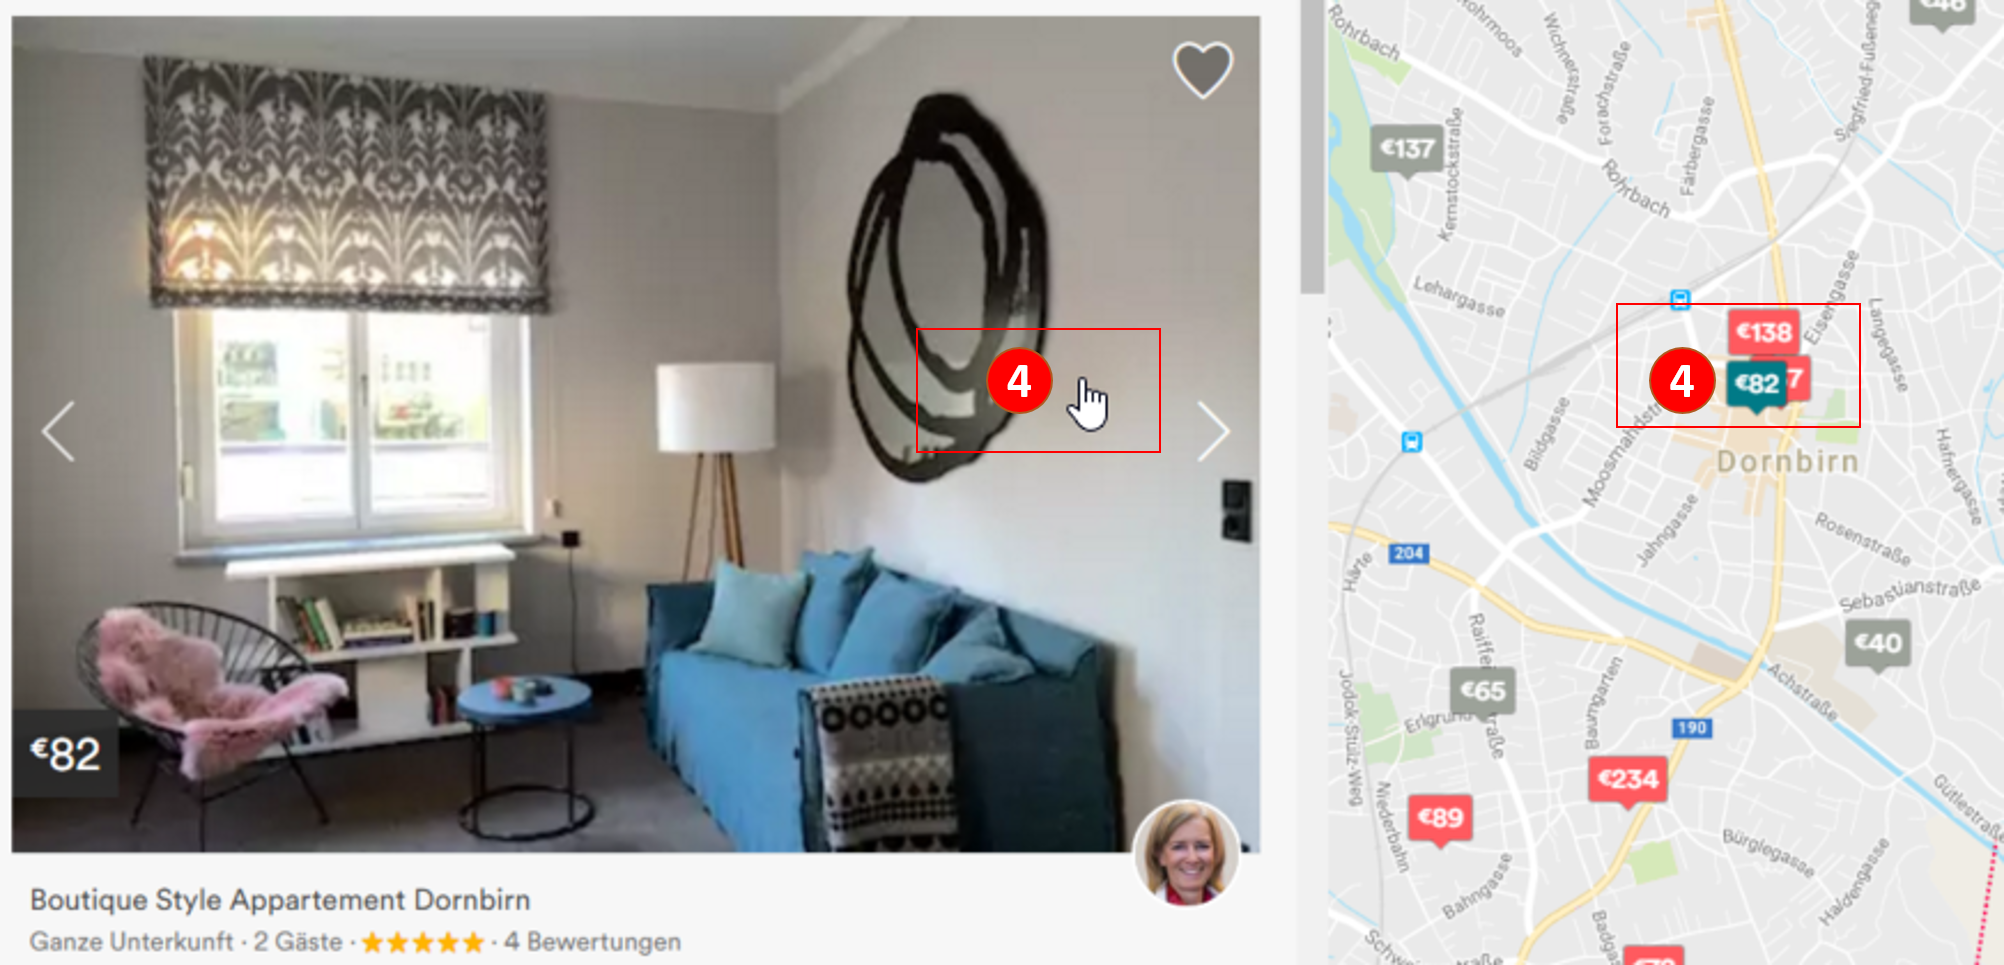
\includegraphics[width=1\linewidth]{img/StandDerTechnik/airbnbDetail}
\caption[Details: Aufbau von Airbnb]{Details: Aufbau von Airbnb (Quelle: eigene Ausarbeitung | Daten und Kartenmaterial: https://www.airbnb.com/ - Stand Sommer 2016)}
\label{fig:airbnbDetail}
\end{figure}

\subsubsection{Zusammenfassung Airbnb}
\label{airbnb:review}


\subsection{Flightradar24}

\end{document}